%
% The first command in your LaTeX source must be the \documentclass command.
\documentclass[sigconf]{acmart}
\usepackage{listings}


%
% defining the \BibTeX command - from Oren Patashnik's original BibTeX documentation.
\def\BibTeX{{\rm B\kern-.05em{\sc i\kern-.025em b}\kern-.08emT\kern-.1667em\lower.7ex\hbox{E}\kern-.125emX}}
    

\copyrightyear{2018}
\acmYear{2018}
\setcopyright{acmlicensed}
\acmConference[Woodstock '18]{Woodstock '18: ACM Symposium on Neural Gaze Detection}{June 03--05, 2018}{Woodstock, NY}
\acmBooktitle{Woodstock '18: ACM Symposium on Neural Gaze Detection, June 03--05, 2018, Woodstock, NY}
\acmPrice{15.00}
\acmDOI{10.1145/1122445.1122456}
\acmISBN{978-1-4503-9999-9/18/06}

%
% These commands are for a JOURNAL article.
%\setcopyright{acmcopyright}
%\acmJournal{TOG}
%\acmYear{2018}\acmVolume{37}\acmNumber{4}\acmArticle{111}\acmMonth{8}
%\acmDOI{10.1145/1122445.1122456}

%
% Submission ID. 
% Use this when submitting an article to a sponsored event. You'll receive a unique submission ID from the organizers
% of the event, and this ID should be used as the parameter to this command.
%\acmSubmissionID{123-A56-BU3}

%
% The majority of ACM publications use numbered citations and references. If you are preparing content for an event
% sponsored by ACM SIGGRAPH, you must use the "author year" style of citations and references. Uncommenting
% the next command will enable that style.
%\citestyle{acmauthoryear}
\setcopyright{none}
\settopmatter{printacmref=false}
\renewcommand\footnotetextcopyrightpermission[1]{}
\pagestyle{plain}
%
% end of the preamble, start of the body of the document source.
\begin{document}

%
% The "title" command has an optional parameter, allowing the author to define a "short title" to be used in page headers.
\title{CSCI 622 Project Report: Phase-3}

%
% The "author" command and its associated commands are used to define the authors and their affiliations.
% Of note is the shared affiliation of the first two authors, and the "authornote" and "authornotemark" commands
% used to denote shared contribution to the research.
\author{Anonymous}
%
% The abstract is a short summary of the work to be presented in the article.
\begin{abstract}
In many new applications that require a database, security is often an afterthought. The integrity of the database is not usually in question until a security incident or a forcing-function such as a compliance audit is required. When there is already significant investment in a database system, switching database implementations or schemas would require non-trivial amounts of work from an engineering team. Common security requirements include having access to an audit trail, providing applications with the least amount of privilege necessary and dynamic code scanning.

To enable easy adoption of common security requirements, an extensible database proxy has been implemented that sits in between the client and a database implementation of choice. This proxy service offers features such as query auditing and access control to help scope access to the database using service accounts and ensure that those access permissions are not being abused. This service can also uncover problems that originate from the developer's implementation such as SQL injection, which can be exposed before hitting the database. Lastly, arbitrary query policies can be enforced to prevent potential attackers from executing scenarios such as dumping an entire database or uncovering data about sensitive users.
\end{abstract}

%
% The code below is generated by the tool at http://dl.acm.org/ccs.cfm.
% Please copy and paste the code instead of the example below.
%
\begin{CCSXML}
<ccs2012>
 <concept>
  <concept_id>10010520.10010553.10010562</concept_id>
  <concept_desc>Computer systems organization~Embedded systems</concept_desc>
  <concept_significance>500</concept_significance>
 </concept>
 <concept>
  <concept_id>10010520.10010575.10010755</concept_id>
  <concept_desc>Computer systems organization~Redundancy</concept_desc>
  <concept_significance>300</concept_significance>
 </concept>
 <concept>
  <concept_id>10010520.10010553.10010554</concept_id>
  <concept_desc>Computer systems organization~Robotics</concept_desc>
  <concept_significance>100</concept_significance>
 </concept>
 <concept>
  <concept_id>10003033.10003083.10003095</concept_id>
  <concept_desc>Networks~Network reliability</concept_desc>
  <concept_significance>100</concept_significance>
 </concept>
</ccs2012>
\end{CCSXML}

% \ccsdesc[500]{Computer systems organization~Embedded systems}
% \ccsdesc[300]{Computer systems organization~Redundancy}
% \ccsdesc{Computer systems organization~Robotics}
% \ccsdesc[100]{Networks~Network reliability}

%%
%% Keywords. The author(s) should pick words that accurately describe
%% the work being presented. Separate the keywords with commas.
\keywords{datasets, anonymization, AWS, cloud, access control, auditing, data harvesting, CLI, API, Postgres}

%% A "teaser" image appears between the author and affiliation
%% information and the body of the document, and typically spans the
%% page.
\maketitle

\section{Introduction}

The two most important cornerstone in any big data application is data security and privacy. Data security is a way of technically safeguarding the data from unauthorized use, while data privacy involved how this safeguarded data is being handled and the sensitivity of the individual attributes that make up the data. Our project's main focus is to explore new and interesting concepts involved in the security and privacy of our data and ultimately design an application that implements these concepts. We also intend to cover and analyze some prevalent issues surrounding the security and privacy of data.

All organizations in this world have sensitive data that should be securely stored and have restricted access. With the world well into the digital age, the majority of the companies hold store data in clouds, privately owned servers and other distributed systems. Data protection, as a result, has become the top priority for any company. Breach of sensitive data could wreak havoc among a company's user-base, it's partners and it's employees. 

However this was not always the case, many companies ignore the security of their data to focus on providing business value. Database and compute configuration often gets ignored, leading to out-of-date software with lots of CVEs or holes in configuration that were ignored during initial setup.

Data security usually involves maintaining the integrity and accessibility of data. It ensures that data is accessed through secure channels and every user needs some level of authorization to view the data. This authorization may involve restrictions in viewing, manipulating or creating the data. On the other hand, data privacy is defined as the way data is handled. Policies must be created by each organization around how data is shared and used, this policy must then be open to the public and must be strictly followed by the company. Privacy policies usually differ with respect to the data that is being collected. Overall, we can say that the higher the sensitivity of data being collected and stored, the stronger should be the data security features and the respective policy. 

In our project, we intend to build a simple application interface or API which will allow us to query a database hosted on a server or cloud. Our plan is to build a system that initially doesn't have any privacy policies and lacks adequate security. We will then show that private data leaks can take place without appropriate data security, and we will show the importance of implementing these concepts mentioned earlier and how they will help secure the database from attacks and unauthorized users. Finally, we will implement the concepts mentioned earlier, show the difference between the initial insecure application and the final secure one. We shall also be exploring data security and privacy concepts such as database auditing, data access controls, application security, database hardening, some common attacks such as SQL injections and also investigate privacy policies in our project.

\section{Design Considerations}

Our project will have an application interface, a database, and a server where the database is hosted which could potentially lead to various data security threats. We shall research security threats involving lack of data audits, poor access control, data management, data leaks, SQL injections, and other application-level threats to data confidence and integrity[3,4,6,7]. 

We shall naturally also focus on the three pillars of data security: 1. Confidentiality, 2. Integrity and 3. Availability. We want to make sure that authorized users can always access data at any time through a secure channel. Hence, access control will be a major part of our system, each user will be a put in an access group with different permissions. For example, admins can create, manipulate, view or delete relations and data within the database, while regular users cannot only view data that they are authorized to but can neither delete existing data nor manipulate it. All data created by regular users must be through the interface. No regular user can be allowed to access the database directly. Different categories of users can always be added in the future with different permissions by the admins. 

We also want to explore different security concepts which include query restrictions, anonymization [5], cloud computing security issues[2], new access control techniques[1], authorization, and database auditing. 

\subsection{Audit and Access Control Considerations}

There are many different things to consider when locking down a database for use in a production environment. Many companies have moved from a monolith approach were there is a single service that has almost root credentials to all systems, to a microservice approach where applications are broken up into many smaller, more focused services. The microservice approach gives security engineers the opportunity to scope down access to the database unlike before because the one application didn't need to be able to read and write to everything in the database. With this, the problem of tracking operations when a security event occurs or when there is a bug is introduced. Having a robust access control and auditing system helps track down and prevent issues with unintended access to data.

Listed below are some concepts that help drive these considerations:
\begin{enumerate}
    \item \textbf{Access Control:} Role-based access control and mandatory access control [1] are some methods we plan on exploring. Applications and developers should only be given enough access to complete their job.
    
    \item \textbf{Query Level Restriction:} There might be users other than admins, such as software engineers or testers who may want to access the database directly. Such users should have restrictions on the queries they can run, as giving every developer opens up many avenues for an attacker to infiltrate.
    
    \item \textbf{Authorization:} Every user will have restricted access to data and will be verified using uniquely identifiable credentials. Additionally, authentication should be done in a secure where others cannot intercept the credentials for their own use.

    \item \textbf{Auditing:} Interactions with the database will be monitored and recorded in the database through the use of an audit log. Ideally, we will want to record the different users who access the database, what data they access, and record the data before any changes (i.e. update). 

   \item \textbf{Data Harvesting Prevention:} Data scraping/harvesting is another security threat that we are looking at, where bots and API crawlers, scrape information from public APIs. Many attackers are looking to harvest as much data as possible to sell to others or hold ransom. 
    
\end{enumerate}

\subsection{Software Development Considerations}

Many security issues are made by software engineers as they use a variety of programming languages and libraries to make queries. Many times it's difficult to scan for these issues as there is so much variety there is not a single technique for how to identify these issues. Below we will discuss a couple of common attacks that are done 

\begin{enumerate}
    \item \textbf{SQL Injection:} users of an application will manipulate input data in order to change the query, exposing information that wouldn't have been shown to the user.
    
    \item \textbf{Cross-site Scripting:} scripting language that can be interpreted by the interface the client uses is inserted into the database, so that it runs on other clients when the fetch the data back, allowing you to control other users usage of the site
\end{enumerate}

\subsection{Database Software, Compute and Network Infrastructure Considerations}

Database systems are something that many people don't want to touch because once they're working they can require little maintenance This can lead to rot of the infrastructure as no one touches it until something is urgently needed. There are many things that must be considered about this area as many times the attacker has the upper-hand as attacks are frequently found and reported, without many organizations updating to the latest patch.

\begin{enumerate}
    \item \textbf{Out of Date Software:} libraries that implement crucial functionality such as encryption or even the database software itself are frequently left at old versions as users don't want to deal with the headache of adapting interfaces to deal with the updates if new features are introduced
    \item \textbf{Sprawling Network Access:} because so many applications have to access a database, many applications leave the server hosting the database application wide open, some times even open to the internet, putting a lot trust into the remote access and authentication software.
\end{enumerate}

\section{Architecture}
\begin{figure}[ht]
      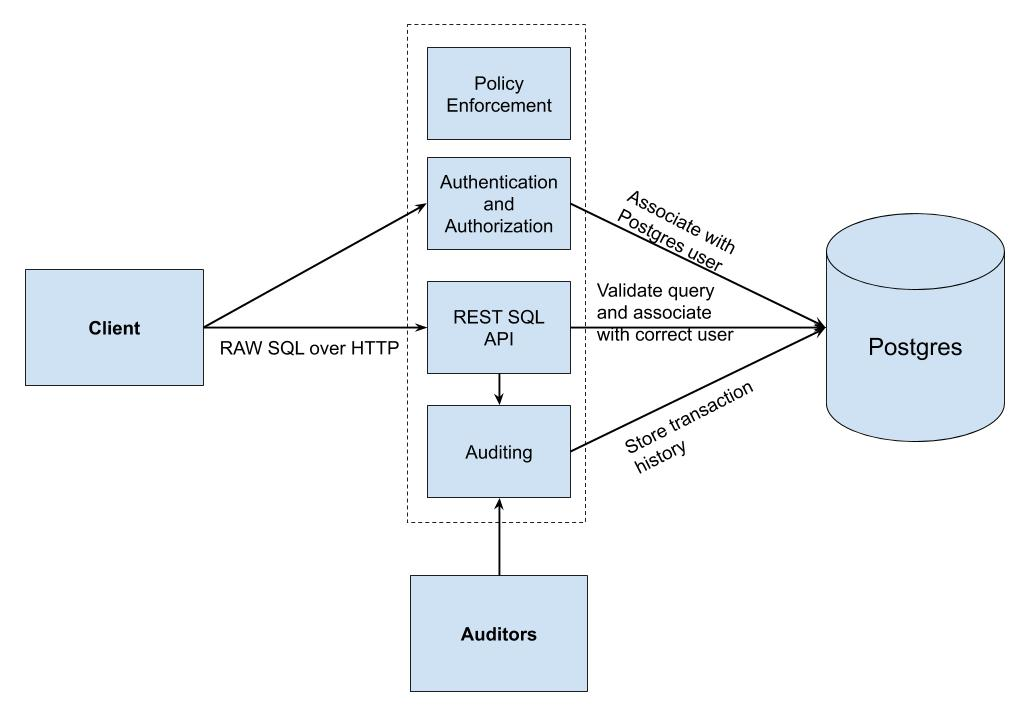
\includegraphics[width=0.5\textwidth]{datasec_project.jpg}
  \caption{System Architecture Diagram}
  \Description{Proxy}
    \label{fig:datasec_project}
\end{figure}

\subsection{Components}

Figure \ref{fig:datasec_project} shows the architecture of our application. It consists of different modules that are scoped to specific tasks, where their composition of functionality forms a complete application.

\begin{enumerate}
    \item \textbf{Client:} Interface used by the end-user to send API requests to perform different operations on the database. The client is password protected, that is, the end-user needs to be authenticated to query the server. Each user is associated with a group with different access privileges. For example, a user associate with the admin group will have access to all the private and public APIs.
    \item \textbf{Authentication and Authorization:} This module acts as the security layer for our application. It validates the user and checks his access restrictions. It ensures that a user indeed has the authorization to query the database, and what kind of privileges the user has on the database. It provides access control over the database to make sure users can only operate on data that they have access to.
    \item \textbf{API:} This is what the client communicates with and is the central ingress to the system. All operations must go through here and it will route requests to the relevant services. Additionally, it will be the main service that interacts with the database after the transaction has been verified with all of the other components in the system.
    \item \textbf{Policy Enforcement:} This module ensures that our security and privacy policies are followed and these policies are made publicly available when a user is created, that is when the user accepts to use the API service. Some potential privacy policies to enforce are data retention, auditing, data loss protection, and encryption. For example, data retention makes sure data is retained for a fixed amount of time before being discarded. A user may have different data retention time concerning the data sensitivity, user preferences and roles. 
    \item \textbf{Auditing:} This service will maintain queryable audit trails, for humans or machines to interact with. The audits usually maintain a log for each user which contains metadata like a user's role, what endpoint access, what operation the user performed on the database and other transaction histories. It also records any errors thrown by the API service or the database, if authentication failed, the reason behind the failure, or if we too many queries were attempted by a single user.
    \item \textbf{Backing Database:} This is our database management system which executes the queries on our data. The implementation should be mostly irrelevant, but drivers for specific implementations can be added to support specific features or add additional security features.  
\end{enumerate}

\section{Implementation}
The below subsections will provide a brief overview of our project plan, discuss the dataset used for testing and technology used to implement the services described in the previous section.

\subsection{Sample Data}

\begin{figure}[ht]
	  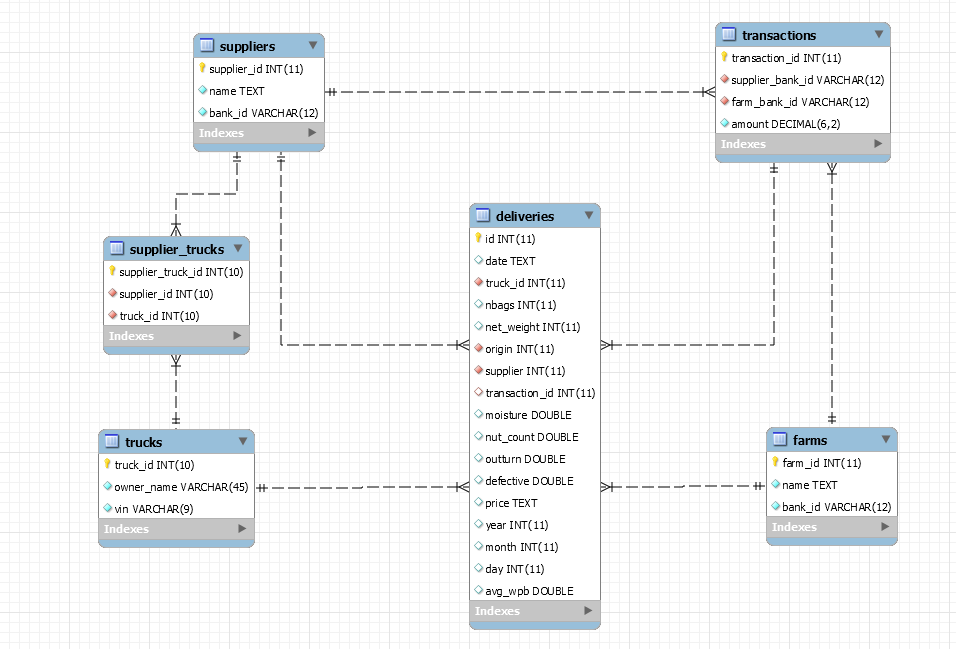
\includegraphics[width=0.5\textwidth]{cashew_erd_updated.png}
  \caption{Relational schema for Cashew Truck Arrivals}
  \Description{Relational schema for cashew truck arrivals dataset}
    \label{fig:cashew_data}
\end{figure}

We will be using a Cashew Truck Arrivals dataset which contains cashew nut deliveries to various suppliers from their respective farm over three years. The data is around 61 KB but we can easily create more data if a larger dataset is needed for testing.

The dataset contains 16 attributes and we use a relational database model to store and access the data. The schema for our relational database is shown in Figure \ref{fig:cashew_data}. In the upcoming phase, we intend to implement integrity constraints and other security features over this schema. There is number of sensitive data fields in our data set like owner\_name, origin\_farm to test with.

\subsection{Application}
 
 The architecture of the application was broken up into many different components allowing the user of this system to select which modules they would like to use or add new modules. Additionally, this allows us to scope SQL credentials to the specific component, providing a more secure interface. Lastly, because these are all separate, they can be written in the language chosen by the implementer, allowing us to easily split up the work between multiple people with different technical backgrounds. 
 
 The main API service communicate with REST over HTTPS to clients. We choose this protocol to provide an easy way to query without providing a complicated client, a user can simply query the API using a shell program such as curl. The primary focus of this service is to query our data. To keep implementation simple data will be returned as JSON, as that is a common format that is expressive and has parser support for almost any language. Queries are encrypted with TLS, to prevent credentials from leaking. This service was written in the Go programming language because of it's large support of many database type and it exposes low level detail while remaining easy to write.
 
 Authorization and Authentication components are integrated directly into the main API and is a wrapping around Postgres's access control functionally with some extra features such as short lived tokens and finer-grained policy enforcement. Queryies are run using this service account to prevent unwanted access on a larger-grained level.
 
 The Auditing module is written to store logs of events that occur to the database and allow to you see the changes. This has been written with a combination of a Postgres hook in order to capture the data that has been captured and a log of all statements that have been executed through an API service that the primary service communicates with. This combination is necessary so that we can capture all statements including SELECT and ALTER TABLE statements which can not be triggered in Postgres directly. All logs are stored in a seperate table as to not interfere with data in the database.
 
 The Policy module is given metadata around the query such as the request itself, the user making the query, statistics about how often the query is made and other data. Imperative policies can then be written and interpreted in order to determine if a query can be executed. This policy is checked by the main API service before executing the query. Some examples of policys include checking the query for SQL injection or making sure that a user belongs to a certain group for querying.

\subsection{Infrastructure}
 We've chosen to host all of our infrastructure in the cloud on AWS's platform. Consumers can access the data through the interface and there will another group of users who can access the database directly as well as through the interface. Access and querying the database is restricted for all users except superusers.
 
 We will testing using a single Postgres instance as our data management system and a database instance. Postgres is open-source with a lot of support and data security extensions that could prove useful for our project. It also provides a very good role-based access control mechanism necessary for our project.
 
 We chose to use a cloud provider solution to ease setup, so we choose AWS's Aurora hosted service. We have created 3 separate users for each member of the team, each user is password protected and have complete permission to modify the database, as well as view, create and delete relations. Additional users can be added as needed to demonstrate the permission restrictions and the security concerns present in the application.

The database is only accessible through a single machine hosted on AWS's EC2 compute infrastructure. This policy is enforced with AWS's security group policies, scoped to the single machine. Our API is hosted on this single machine which has locked down SSH access, only accessible with the the three X. 509 certificates issued to each of our group's members. All ingress to the API will be handled through AWS's Application Load Balancer to not expose identifiable information about the machine.

\section{Lessons Learned}

We are currently still evaluating our lessons learned and will  have a detailed report available for the final phase of the project, but we do  have a few notes that we have noticed:

\begin{enumerate}
    \item SQL protocols are heavily optimized and introducing middleware has a large impact on the latency of the query, this may be unacceptable for many business use cases that require high throughput of data from their systems
    \item The distributed nature of the project made it easy to split of the work, but difficult to deploy and possibly manage by ourselves and others
    \item There are a lot of data you want to capture while auditing and the tables grow very fast, so some smart trimming must be done to prevent this from getting out of control
\end{enumerate}

\section{Current Status and Future Plan}

We have currently implemented access control features and API routes to query the database using a HTTP interface through a central API service written in Go. This application enforces small the small hard-coded policies such as the correct user is making the query.

We plan to finish implementing auditing functionality into the code. We wish to record changes in the tables so that they can later be audited (i.e. transaction amounts).  While Postgres natively supports auditing of most CRUD operations through the user of triggers, it does not support the recording of SELECT statements which we show us if any user on the database executed an undesirable query (i.e. searching for PII not belonging to the user). PGAudit is an example tool we plan on using for auditing these queries to ensure that all activity on the database is recorded.

This tool could be taken much further to add more modules such as dynamically scoped roles which determine w hat access a application needs based  on the queries it uses. Another possible extension is automatic alerting of suspicious activity and lock down specific queries to prevent unwanted access to the database.

The current modules could also be extended to provide more metadata for writing policies against and putting into the audit trail. The more metadata that is available the easier it will be to correlate it to security events or automatically discover them.

Lastly, we recognize the impact on performance this middleware has and there could be many optimizations made to support SQL protocols natively, instead of translating them into JSON responses.

\begin{thebibliography}{9}

\bibitem{Data Security} 
    Elisa Bertino,
    \textit{ "Data mining with big data," in Data \& Knowledge Engineering 25 (1998) 199-216}. 

\bibitem{Data Security and Privacy Protection Issues in Cloud Computing} 
 D. Chen and H. Zhao,
     \textit{ "Data Security and Privacy Protection Issues in Cloud Computing," 2012 International Conference on Computer Science and Electronics Engineering, Hangzhou, 2012, pp. 647-651.}
     
\bibitem{Security of Big Data: A Review} 
    R. Bhatia and M. Sood,
    \textit{"Security of Big Data: A Review," 2018 Fifth International Conference on Parallel, Distributed and Grid Computing (PDGC), Solan Himachal Pradesh, India, 2018, pp. 182-186.}
     
\bibitem{Security and privacy for big data: A systematic literature review} 
    B. Nelson and T. Olovsson,
     \textit{ "Security and privacy for big data: A systematic literature review," 2016 IEEE International Conference on Big Data (Big Data), Washington, DC, 2016, pp. 3693-3702.}. 
     
 \bibitem{Making Big Data, Privacy, and Anonymization Work Together in the Enterprise: Experiences and Issues} 
    Sedayao, Jeff \& Bhardwaj, Rahul \& Gorade, Nakul.
    \textit{ "Making Big Data, Privacy, and Anonymization Work Together in the Enterprise: Experiences and Issues," Proceedings - 2014 IEEE International Congress on Big Data, BigData Congress 2014. 10.1109/BigData.Congress.2014.92. }. 

\bibitem{Big Data - Security and Privacy} 
    E. Bertino,
    \textit{ "Big Data - Security and Privacy," 2015 IEEE International Congress on Big Data, New York, NY, 2015, pp. 757-761.}. 

\bibitem{Big data privacy: a technological perspective and review} 
    Jain, P., Gyanchandani, M. \& Khare, N.
    \textit{Big data privacy: a technological perspective and review. J Big Data 3, 25 (2016). https://doi.org/10.1186/s40537-016-0059-y}



\end{thebibliography}

\end{document}
